\documentclass[conference]{IEEEtran}
\IEEEoverridecommandlockouts

\usepackage{cite}
\usepackage{amsmath,amssymb,amsfonts}
\usepackage{graphicx}
\usepackage{textcomp}
\usepackage{xcolor}
\usepackage{booktabs}
\usepackage{url}
\usepackage{microtype}
\usepackage{balance}

\setlength{\textfloatsep}{6pt plus 1pt minus 1pt}
\setlength{\dbltextfloatsep}{6pt plus 1pt minus 1pt}
\setlength{\floatsep}{5pt plus 1pt minus 1pt}
\setlength{\dblfloatsep}{5pt plus 1pt minus 1pt}
\setlength{\intextsep}{5pt plus 1pt minus 1pt}

\makeatletter
\newcommand{\linebreakand}{%
  \end{@IEEEauthorhalign}
  \hfill\mbox{}\par
  \mbox{}\hfill\begin{@IEEEauthorhalign}
}
\makeatother

\begin{document}

\title{Explainable AI for Lithography Hotspot Detection: A Multi-Method XAI Analysis}

\author{
\IEEEauthorblockN{Allen Joe A}
\IEEEauthorblockA{\textit{School of Electronics Engineering (SENSE)} \\
\textit{VIT Chennai}\\
Chennai, India \\
allenjoe.a2024@vitstudent.ac.in}
\and
\IEEEauthorblockN{R. Naga Arjun}
\IEEEauthorblockA{\textit{School of Electronics Engineering (SENSE)} \\
\textit{VIT Chennai}\\
Chennai, India \\
nagaarjun.r2024@vitstudent.ac.in}
\linebreakand
\IEEEauthorblockN{Prasiddh Kumar Saha}
\IEEEauthorblockA{\textit{School of Electronics Engineering (SENSE)} \\
\textit{VIT Chennai}\\
Chennai, India \\
prasiddh.2024@vitstudent.ac.in}
\and
\IEEEauthorblockN{Chitluri Sohan}
\IEEEauthorblockA{\textit{School of Electronics Engineering (SENSE)} \\
\textit{VIT Chennai}\\
Chennai, India \\
sohan.chitluri2024@vitstudent.ac.in}
}

\maketitle

\begin{abstract}
Lithography hotspots are layout regions prone to printing defects such as opens and shorts caused by optical lithography diffraction limitations and aggressive IC pitch scaling. This work develops an explainable-AI (XAI) framework for lithography hotspot detection using convolutional neural networks (CNNs) trained independently on the five real ICCAD-12 benchmark datasets. A lightweight reference CNN baseline ($\approx 12.9\text{k}$ parameters) is compared with an XAI-ready variant ($\approx 128.3\text{k}$ parameters) designed to preserve spatial feature representations through three named convolutional stages. The evaluation pipeline includes rigorous 3-way train/validation/test split isolation, leakage correction, pipeline-level comparison, and class-imbalance ablations. Four post-hoc attribution methods---Grad-CAM, closed-form Grad-CAM++, LayerCAM, and occlusion sensitivity---are evaluated across 57 representative predictions covering true positive (TP), true negative (TN), false positive (FP), and false negative (FN) outcomes, supplemented by independently regenerated clean-checkpoint attribution maps. Quantitative 2D raster-morphology validation and occlusion cross-checks demonstrate that attribution fidelity is method- and outcome-dependent: LayerCAM and occlusion provide consistent layout sensitivity, whereas Grad-CAM is effective primarily on true positives and degrades under gradient cancellation or feature collapse. The classification and multi-method XAI pipelines are verified on clean splits; future work targets foundry DRC rule validation and optical lithography simulation.
\end{abstract}

\begin{IEEEkeywords}
Explainable artificial intelligence, lithography hotspot detection, convolutional neural network, Grad-CAM, Grad-CAM++, LayerCAM, occlusion sensitivity, ICCAD-12.
\end{IEEEkeywords}

\section{Introduction}
Photolithography is the dominant technique for patterning integrated circuits, but as feature sizes shrink below the lithography wavelength, certain layout patterns become susceptible to printing failures known as lithography hotspots. Typical failures include pinching that can produce open circuits and bridging that can produce short circuits.

Physics-based lithography simulation can identify such hotspots accurately, but exhaustive simulation is computationally expensive for full-chip verification. This motivates machine-learning based detectors that operate directly on layout clip images. The real ICCAD-12 benchmark provides a standard basis for evaluating such detectors and contains five independent benchmark sets with severe and unequal class imbalance.

A CNN can provide a fast binary decision, but its black-box nature limits a designer's ability to understand why a layout was classified as a hotspot. The research question of this project is therefore: \textit{can explainable-AI techniques identify the layout regions or features that contribute most strongly to hotspot classification, and are those highlighted regions technically meaningful?}

The project is organized into two connected stages. First, a lightweight CNN is trained independently on the five real ICCAD-12 benchmark datasets for hotspot (HS) versus non-hotspot (NHS) classification. Second, the trained classifier is analyzed using multiple post-hoc attribution methods. The latest stage extends the original Grad-CAM plan to Grad-CAM++, LayerCAM, and occlusion sensitivity so that gradient-based explanations can be cross-checked against an independent forward-pass method.

The completed investigation contributes:
\begin{enumerate}
    \item Independent per-benchmark CNN training on the real ICCAD-12 datasets;
    \item An XAI-ready architecture with preserved spatial feature maps;
    \item Explicit handling and ablation of severe class imbalance;
    \item Identification and empirical quantification of test/validation leakage;
    \item Comprehensive side-by-side performance comparison;
    \item Four-method XAI analysis across 57 representative predictions and regenerated clean figures; and
    \item Quantitative 2D raster morphology and occlusion-based validation of explanations.
\end{enumerate}

\section{Related Work}
Verma et al.~\cite{verma2026} compare VGG16-based transfer learning followed by SVM, Random Forest, or $k$-NN classification against a lightweight CNN trained from scratch on ICCAD-12. The lightweight CNN is reported to achieve higher balanced accuracy and faster inference, motivating its use as the reference baseline in this work. Borisov and Scheible~\cite{borisov2018} previously proposed a lightweight CNN design for lithography hotspot detection, while Liao et al.~\cite{liao2022} and Yang et al.~\cite{yang2017} studied transfer learning and shallow-to-deep learning approaches.

Class Activation Mapping (CAM) introduced class-discriminative localization using global-average pooling~\cite{zhou2016}. Grad-CAM generalized this approach using gradients of a target-class score with respect to convolutional feature maps~\cite{selvaraju2017}. Grad-CAM++~\cite{chattopadhyay2018} uses higher-order gradient information to improve localization, while LayerCAM~\cite{jiang2021layercam} applies spatially varying gradient weighting at individual feature-map locations.

Occlusion sensitivity provides an independent attribution mechanism: input regions are systematically masked and the resulting change in the target-class score is measured. This makes occlusion useful for checking whether gradient-based maps reflect actual model sensitivity rather than gradient-specific artifacts.

LithoExp~\cite{jiang2025lithoexp} is closely related because it addresses explainability and defect localization in lithographic hotspot detection. The present work differs by applying four post-hoc attribution methods to a classifier whose spatial representation is deliberately retained for XAI, and by quantitatively comparing the resulting maps against geometric layout proxies and occlusion sensitivity.

\section{Dataset and Class-Imbalance Analysis}

\subsection{ICCAD-12 Dataset}
All primary experiments use the five real ICCAD-12 benchmarks, evaluated strictly independently. Layout clips are loaded from the benchmark \texttt{train\_hs}, \texttt{train\_nhs}, \texttt{test\_hs}, and \texttt{test\_nhs} partitions, resized to $224\times224$, and rescaled to $[0,1]$. Table~\ref{tab:dataset} reports the complete per-benchmark image counts and the class-imbalance ratios for both training and test partitions.

\begin{table}[htbp]
\caption{Per-Benchmark Class Distribution and Imbalance Ratios}
\label{tab:dataset}
\centering
\setlength{\tabcolsep}{3pt}
\begin{tabular}{lcccccc}
\toprule
 & \multicolumn{3}{c}{\textbf{Train Partition}} & \multicolumn{3}{c}{\textbf{Test Partition}} \\
\cmidrule(lr){2-4} \cmidrule(lr){5-7}
\textbf{Benchmark} & \textbf{HS} & \textbf{NHS} & \textbf{NHS:HS} & \textbf{HS} & \textbf{NHS} & \textbf{NHS:HS} \\
\midrule
\textbf{ICCAD-1} & 99 & 340 & 3.4:1 & 226 & 4,679 & 20.7:1 \\
\textbf{ICCAD-2} & 174 & 5,285 & 30.4:1 & 498 & 41,298 & 82.9:1 \\
\textbf{ICCAD-3} & 909 & 4,643 & 5.1:1 & 1,808 & 46,333 & 25.6:1 \\
\textbf{ICCAD-4} & 95 & 4,452 & 46.9:1 & 177 & 31,890 & 180.2:1 \\
\textbf{ICCAD-5}* & 26 & 2,716 & 104.5:1 & 41 & 19,327 & 471.4:1 \\
\bottomrule
\end{tabular}
\vspace{1mm}
\begin{flushleft}
\footnotesize{*Note: In ICCAD-5 test NHS, $\approx 89\%$ of files follow a \texttt{.pngN.png} pattern representing synthetic replicates from $\approx 3$ unique base rasters per stem, rather than independent layout clips.}
\end{flushleft}
\end{table}

As documented in Table~\ref{tab:dataset}, every benchmark is heavily dominated by non-hotspot clips. The training imbalance spans from 3.4:1 (ICCAD-1) to 104.5:1 (ICCAD-5), while the test imbalance ranges from 20.7:1 (ICCAD-1) to 471.4:1 (ICCAD-5). A trivial classifier that unconditionally predicts non-hotspot would achieve over 99.7\% accuracy on ICCAD-5 while detecting zero hotspots. Consequently, balanced accuracy, sensitivity, specificity, precision, and F1-score are reported to fairly evaluate hotspot detection.

\subsection{Preprocessing and Augmentation}
All models were trained on the real ICCAD-12 benchmark data. For the latest XAI pipeline, layout clips are resized from their native $1200\times1200$ raster representation to $224\times224$ and rescaled to $[0,1]$. No rotation, flip, or other augmentation is used in the primary baseline or XAI-ready training runs, so both models operate on the same un-augmented per-benchmark train/test partitions.

\subsection{Class-Imbalance Handling}
Two imbalance strategies were investigated. The baseline uses no class weighting. The XAI-ready pipeline initially used inverse-frequency class weighting and selected checkpoints using balanced accuracy on a validation split. A dedicated ICCAD-5 ablation later showed that the loss-reweighted condition was responsible for a feature-collapse failure mode; balanced mini-batch sampling did not show the same collapse. Some ablation scripts still require clean-split re-verification, so those results are treated as provisional.

\section{Methodology}

\subsection{Baseline CNN}
The baseline network reproduces the reference lightweight-CNN design~\cite{verma2026, borisov2018}. It uses stacked $3\times3$ convolutional layers with ELU activations and batch normalization, max-pooling, and a flatten-and-fully-connected classification head with dropout. With $224\times224$ input, the baseline reduces the spatial representation to approximately a $15\times15$ feature grid before flattening. This aggressive spatial reduction is important when interpreting the coarseness of its activation maps.

\subsection{Proposed GAP-CNN}
The proposed XAI-ready CNN keeps comparable convolutional depth but deliberately preserves spatial information for explanation. Three named stages are retained: \texttt{conv\_early\_2} ($112\times112\times16$), \texttt{conv\_mid\_2} ($56\times56\times24$), and \texttt{conv\_final\_2} ($28\times28\times32$). The \texttt{conv\_final\_2} feature map is the primary attribution target for Grad-CAM, Grad-CAM++, LayerCAM, and the corresponding cross-check analysis. The model then uses a late max-pool, flatten, Dropout(0.3), Dense(16, ReLU), and Dense(1, sigmoid) head.

\begin{table*}[t]
\caption{Architectural Comparison of the Baseline and Proposed XAI-Ready CNN}
\label{tab:architecture}
\centering
\setlength{\tabcolsep}{4pt}
\begin{tabular}{p{0.20\textwidth}p{0.37\textwidth}p{0.37\textwidth}}
\toprule
\textbf{Stage / Attribute} & \textbf{Baseline CNN} & \textbf{Proposed XAI-Ready CNN} \\
\midrule
\textbf{Input Format} & $224\times224\times3$ RGB & $224\times224\times3$ RGB \\
\textbf{Spatial Feature Stages} & Downsampled aggressively to $\approx 15\times15$ & Preserved stages: $112\times112\times16$, $56\times56\times24$, $28\times28\times32$ \\
\textbf{Convolutional Backbone} & Lightweight stacked $3\times3$ ELU layers & Three named spatially-preserved stages \\
\textbf{Classification Head} & Flatten + Fully Connected + Dropout(0.3) & Late max-pool + Flatten + Dropout(0.3) + Dense(16) + Sigmoid \\
\textbf{Attribution Target Layer} & Penultimate dense representation & \texttt{conv\_final\_2} ($28\times28\times32$) \\
\textbf{Design Purpose} & Reference baseline~\cite{verma2026} & High-resolution classification + multi-method XAI \\
\textbf{Parameter Count} & 12,873 ($\approx 12.9\text{k}$) & 128,321 ($\approx 128.3\text{k}$) \\
\bottomrule
\end{tabular}
\end{table*}

The architectural choice treats explainability as a design constraint: the classifier must retain spatially meaningful feature maps rather than discarding almost all location information before the classification head. The Dense(16) layer following late pooling ($14\times14\times32$) accounts for 100,368 of the 128,321 parameters in the XAI model. Importantly, the comparison between the baseline and proposed model evaluates two distinct end-to-end training and inference pipelines rather than an isolated architecture-only ablation.

\subsection{Training Configuration}
Both models are trained independently on the five real ICCAD-12 benchmarks with batch size 32 and the Nadam optimizer. The baseline uses the fixed per-benchmark epoch budget (5--10 epochs) and final-epoch weights without class weighting, reproducing the reference implementation~\cite{verma2026}. In contrast, the XAI-ready pipeline employs inverse-frequency class weighting ($w_c = N / (2 N_c)$) and selects the best checkpoint based on validation balanced accuracy computed on a stratified 15\% split carved out from the training set. The official test split is evaluated only once after final checkpoint selection, avoiding optimistic data leakage.

\begin{table}[htbp]
\caption{Training Configuration for Baseline and XAI-Ready CNN}
\label{tab:training_config}
\centering
\setlength{\tabcolsep}{3pt}
\begin{tabular}{p{0.36\columnwidth}p{0.58\columnwidth}}
\toprule
\textbf{Parameter} & \textbf{Configuration} \\
\midrule
\textbf{Optimizer} & Nadam \\
\textbf{Batch size} & 32 \\
\textbf{Input dimensions} & $224\times224\times3$ RGB \\
\textbf{Baseline epochs} & 5 / 5 / 10 / 10 / 10 (per benchmark, final epoch) \\
\textbf{Baseline loss} & Standard binary cross-entropy (unweighted) \\
\textbf{XAI loss} & Inverse-frequency class-weighted BCE \\
\textbf{XAI checkpointing} & Best validation balanced accuracy \\
\textbf{Validation split} & 15\% stratified carve-out from training set \\
\textbf{Test evaluation} & Evaluated once on held-out test partition \\
\bottomrule
\end{tabular}
\end{table}

\section{Evaluation Metrics}
With hotspot as the positive class, the confusion matrix contains true positives (TP), false positives (FP), true negatives (TN), and false negatives (FN). The standard metrics used throughout the project are:
\begin{equation}
\text{Precision} = \frac{\text{TP}}{\text{TP} + \text{FP}}
\end{equation}
\begin{equation}
\text{Recall (Sensitivity)} = \frac{\text{TP}}{\text{TP} + \text{FN}}
\end{equation}
\begin{equation}
\text{Specificity} = \frac{\text{TN}}{\text{TN} + \text{FP}}
\end{equation}
\begin{equation}
\text{F1} = \frac{2 \times \text{Precision} \times \text{Recall}}{\text{Precision} + \text{Recall}}
\end{equation}
\begin{equation}
\text{Balanced Accuracy} = \frac{\text{Sensitivity} + \text{Specificity}}{2}
\end{equation}

Balanced accuracy is treated as the primary summary metric because it gives equal weight to hotspot sensitivity and non-hotspot specificity regardless of class imbalance. Precision reflects review overload in physical design, while recall reflects defect avoidance.

\section{Experimental Results}

\subsection{Proposed GAP-CNN Results and Pipeline Comparison}
Table~\ref{tab:main_results} reports the complete per-benchmark comparison of the baseline and proposed XAI-ready CNN across balanced accuracy, recall, precision, and F1-score on clean test splits. Across all five benchmarks, the baseline achieves an average balanced accuracy of 0.9363, while the clean-split XAI-ready model achieves 0.9319. The small difference demonstrates that preserving spatial feature maps does not compromise overall balanced accuracy.

\begin{table*}[t]
\caption{Comprehensive Comparison: Baseline CNN vs. Proposed XAI-Ready CNN on Clean Splits}
\label{tab:main_results}
\centering
\begin{tabular}{lcccccccc}
\toprule
 & \multicolumn{4}{c}{\textbf{Baseline CNN (Unweighted, Final Epoch)}} & \multicolumn{4}{c}{\textbf{Proposed XAI-Ready CNN (Class-Weighted, Val-Selected)}} \\
\cmidrule(lr){2-5} \cmidrule(lr){6-9}
\textbf{Benchmark} & \textbf{Bal.~Acc.} & \textbf{Recall} & \textbf{Precision} & \textbf{F1} & \textbf{Bal.~Acc.} & \textbf{Recall} & \textbf{Precision} & \textbf{F1} \\
\midrule
\textbf{ICCAD-1} & 0.8851 & 0.9867 & 0.1804 & 0.3051 & 0.8743 & 0.9735 & 0.1730 & 0.2937 \\
\textbf{ICCAD-2} & 0.9893 & 0.9900 & 0.5119 & 0.6749 & 0.9841 & 0.9819 & 0.4618 & 0.6281 \\
\textbf{ICCAD-3} & 0.9672 & 0.9773 & 0.4707 & 0.6354 & 0.9508 & 0.9829 & 0.3208 & 0.4837 \\
\textbf{ICCAD-4} & 0.8578 & 0.7175 & 0.6720 & 0.6940 & 0.9534 & 0.9492 & 0.1107 & 0.1983 \\
\textbf{ICCAD-5} & 0.9822 & 0.9756 & 0.1556 & 0.2685 & 0.8969 & 0.8049 & 0.1336 & 0.2292 \\
\midrule
\textbf{Average} & \textbf{0.9363} & \textbf{0.9294} & \textbf{0.3981} & \textbf{0.5156} & \textbf{0.9319} & \textbf{0.9385} & \textbf{0.2400} & \textbf{0.3666} \\
\bottomrule
\end{tabular}
\end{table*}

However, the precision and F1 trade-offs differ significantly between pipelines. The XAI-ready pipeline maintains higher average hotspot recall (0.9385 vs. 0.9294) but incurs substantially lower precision (0.2400 vs. 0.3981) and average F1 (0.3666 vs. 0.5156). This behavior directly reflects the inverse-frequency loss weighting, which heavily penalizes false negatives on minority hotspots at the expense of generating more false positives in imbalanced regimes (most acutely on ICCAD-4, where precision falls from 67.2\% to 11.1\%). This confirms that decision-threshold calibration on validation data is necessary to restore precision balance.

\subsection{Baseline-versus-Proposed Comparison and Leakage Correction}
The baseline-versus-proposed comparison is now available from the latest training runs. Table~\ref{tab:leakage} reports the per-benchmark comparison of the XAI-ready CNN before and after test/validation leakage correction.

\begin{table}[htbp]
\caption{XAI-Ready CNN Balanced Accuracy Before and After Leakage Correction}
\label{tab:leakage}
\centering
\begin{tabular}{lccc}
\toprule
\textbf{Benchmark} & \textbf{Leaked BA} & \textbf{Clean BA} & \textbf{$\Delta$ (pp)} \\
\midrule
\textbf{ICCAD-1} & 0.8935 & 0.8743 & $-1.92$ \\
\textbf{ICCAD-2} & 0.9314 & 0.9841 & $+5.27$ \\
\textbf{ICCAD-3} & 0.9641 & 0.9508 & $-1.32$ \\
\textbf{ICCAD-4} & 0.9430 & 0.9534 & $+1.04$ \\
\textbf{ICCAD-5} & 0.9501 & 0.8969 & $-5.32$ \\
\midrule
\textbf{Average} & \textbf{0.9364} & \textbf{0.9319} & \textbf{$-0.45$} \\
\bottomrule
\end{tabular}
\end{table}

\begin{figure}[htbp]
\centering
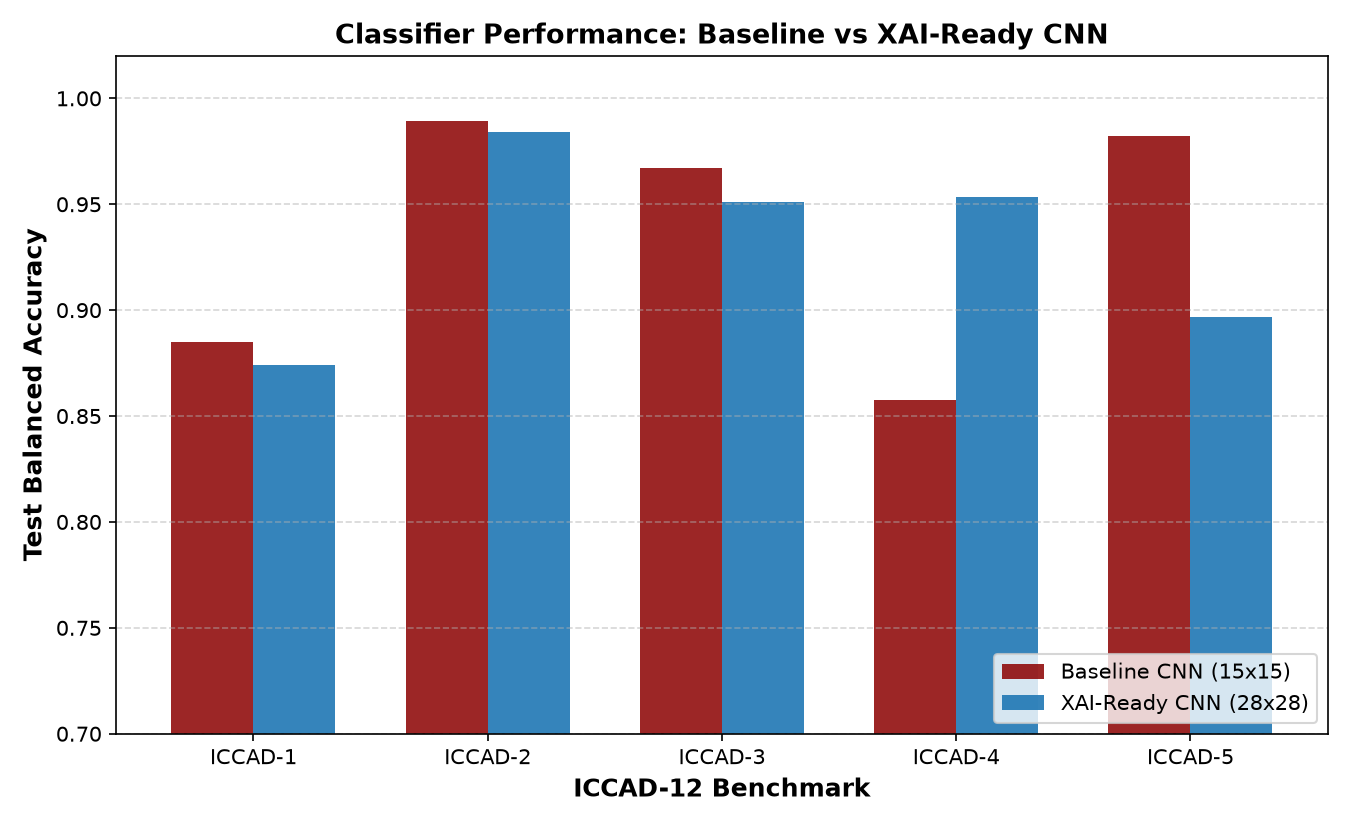
\includegraphics[width=0.88\columnwidth]{figures/image6.png}
\caption{Baseline versus proposed XAI-ready CNN balanced accuracy across the five ICCAD-12 benchmarks.}
\label{fig:comparison_bar}
\end{figure}

\subsection{Cross-Benchmark Pooling Ablation}
As a controlled ablation, a ResNet-18 backbone adapted to single-channel input was trained on all five real ICCAD-12 benchmarks pooled into one training set and evaluated separately on each benchmark's test split. The pooled model produced unusually high detection rates and ROC-AUC values across all five benchmarks (Table~\ref{tab:resnet_pooled}).

\begin{table*}[t]
\caption{ResNet-18 Trained on All Five Benchmarks Pooled Together and Evaluated Per Benchmark}
\label{tab:resnet_pooled}
\centering
\begin{tabular}{lccccc}
\toprule
\textbf{Benchmark} & \textbf{Test Samples ($n$)} & \textbf{Detection Rate (Recall)} & \textbf{False Alarm Rate} & \textbf{ROC-AUC} \\
\midrule
\textbf{ICCAD-1} & 29,430 & 94.10\% & 1.82\% & 0.9897 \\
\textbf{ICCAD-2} & 250,776 & 98.53\% & 0.15\% & 0.9998 \\
\textbf{ICCAD-3} & 288,846 & 96.91\% & 1.47\% & 0.9930 \\
\textbf{ICCAD-4} & 192,402 & 93.50\% & 0.82\% & 0.9675 \\
\textbf{ICCAD-5} & 116,208 & 91.87\% & 0.20\% & 0.9994 \\
\midrule
\textbf{Total Pooled} & \textbf{877,662} & --- & --- & --- \\
\bottomrule
\end{tabular}
\end{table*}

\begin{figure}[htbp]
\centering
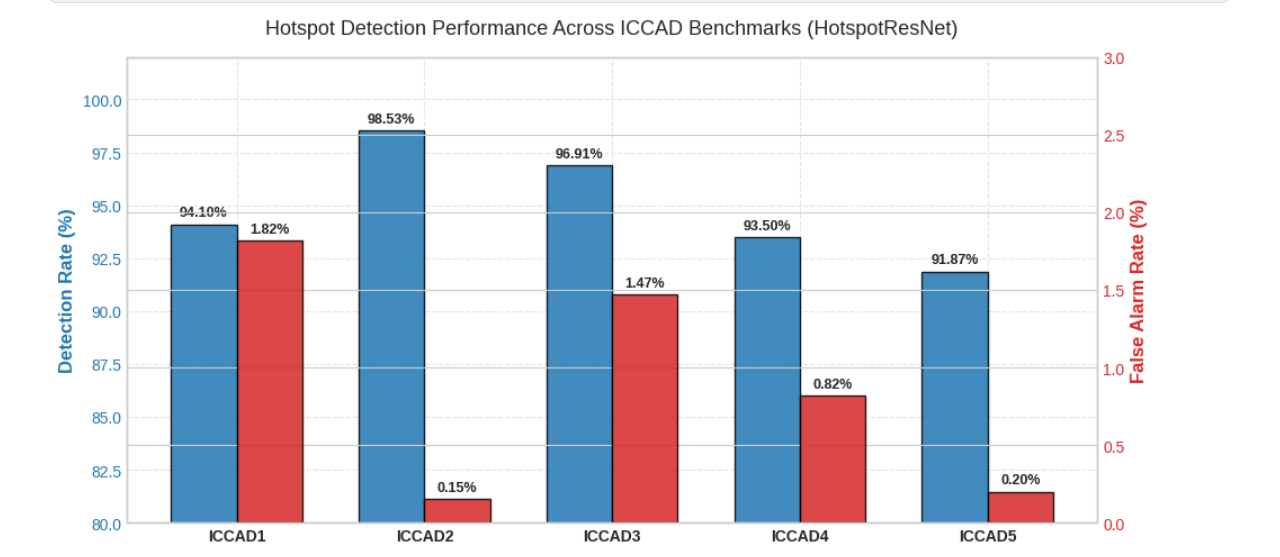
\includegraphics[width=\columnwidth]{figures/image1.png}
\caption{Detection rate and false-alarm rate per benchmark for the pooled-training ResNet-18 ablation.}
\label{fig:pooled_bar}
\end{figure}

However, these figures must be interpreted with extreme caution and are retained strictly as a methodological ablation rather than evidence of superior generalization. Forensic inspection reveals two critical methodological caveats:
\begin{enumerate}
    \item \textbf{Exact $6\times$ Expansion via Transformed Copies:} The test sample sizes ($n$) are exactly $6\times$ larger than the raw test sets (e.g., ICCAD-1: $4,905 \times 6 = 29,430$; ICCAD-2: $41,796 \times 6 = 250,776$; totaling 877,662 test clips). Each clip was expanded via six dihedral rotation and reflection transforms. If offline augmentation was applied without clip-level disjoint grouping, transformed copies of the same pattern may have crossed train and test partitions.
    \item \textbf{Cross-Benchmark Motif Leakage:} Pooling layout clips across diverse technology nodes blends design rules, increasing near-duplicate pattern overlap across benchmarks.
\end{enumerate}
Consequently, independent benchmark training without cross-pooling or test-set transformation remains our primary scientific methodology.

\begin{figure*}[t]
\centering
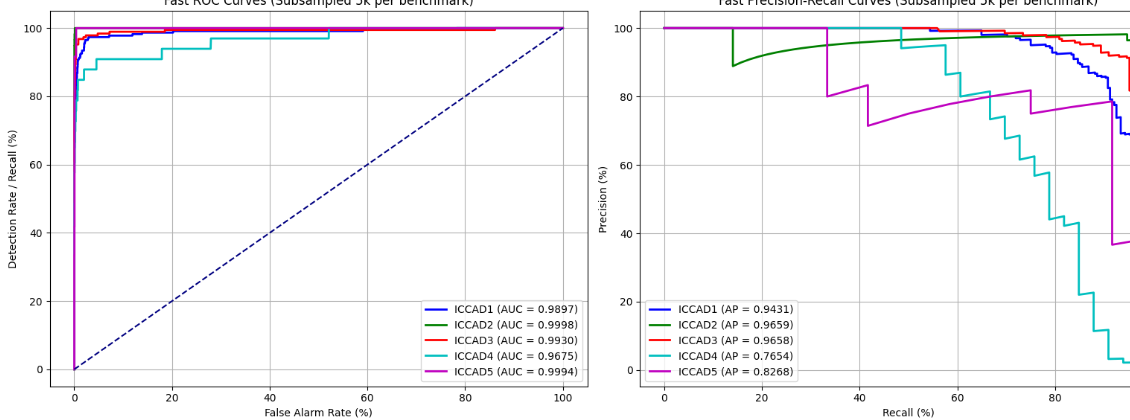
\includegraphics[width=0.92\textwidth]{figures/image2_cropped.png}
\caption{ROC and precision-recall curves for the pooled-training ResNet-18 evaluated separately on each benchmark.}
\label{fig:pooled_roc_pr}
\end{figure*}

\section{Additional Evaluation and Pipeline Smoke-Testing}

\subsection{Pooled ResNet-18 ROC and Precision-Recall Curves}
The ROC and precision-recall curves shown in Fig.~\ref{fig:pooled_roc_pr} document the pooled ResNet-18 ablation. They illustrate why near-perfect ROC curves (AUC $> 0.999$) warrant scrutiny when data expansion and cross-benchmark pooling are involved.

\subsection{Evaluation Pipeline Diagnostic Smoke-Test}
To verify the internal correctness of the evaluation codebase---specifically confusion-matrix extraction, ROC/PR curve plotting, and threshold-optimization sweeps---a smoke-test was executed on a diagnostic 5,000-clip synthetic fixture (\texttt{ICCAD1 Synthetic}, comprising 256 HS and 4,744 NHS clips; see Figs.~\ref{fig:val_roc_pr}--\ref{fig:val_cm} and Table~\ref{tab:pipeline_val}).

\begin{figure}[htbp]
\centering
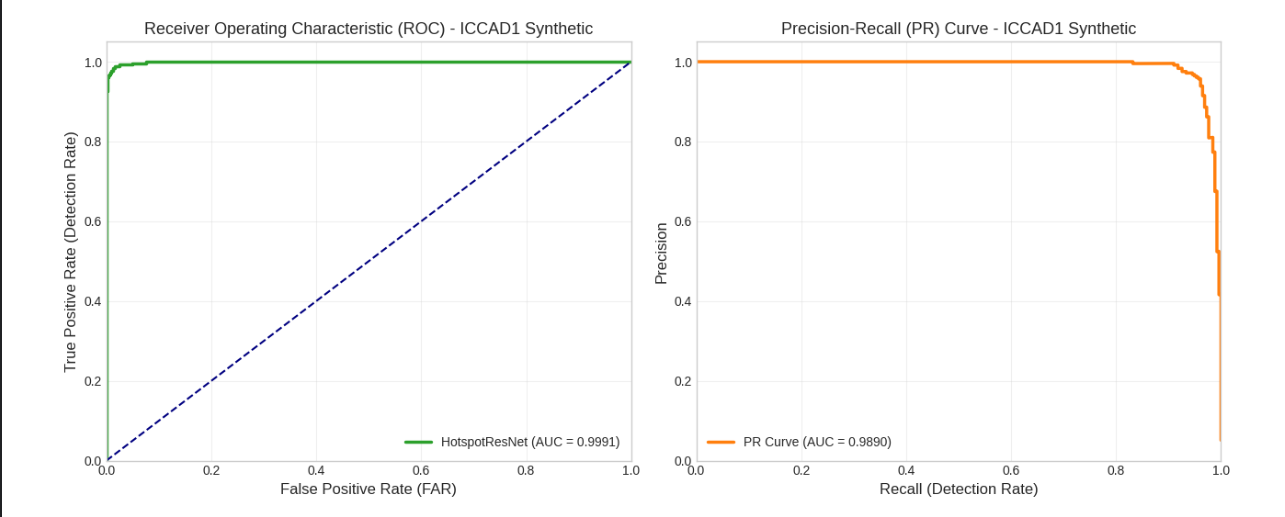
\includegraphics[width=0.95\columnwidth]{figures/image3.png}
\caption{ROC and PR curves generated during evaluation pipeline smoke-testing on the 5,000-sample \texttt{ICCAD1 Synthetic} diagnostic fixture.}
\label{fig:val_roc_pr}
\end{figure}

\begin{figure}[htbp]
\centering
\begin{minipage}[b]{0.48\columnwidth}
\centering
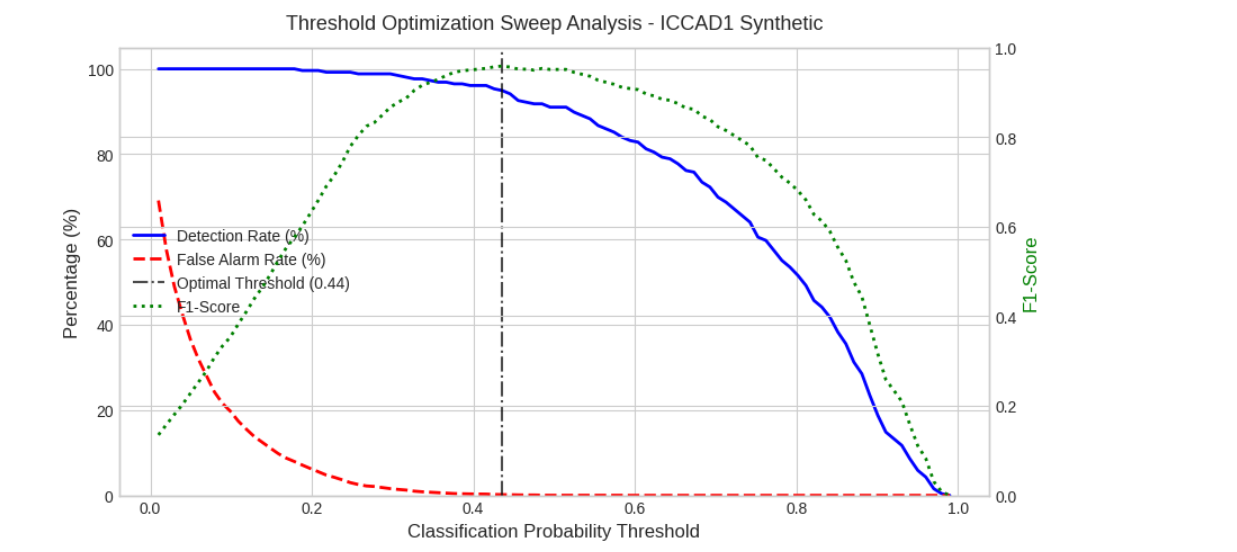
\includegraphics[width=\textwidth]{figures/image4.png}
\caption{Threshold sweep on diagnostic fixture; optimum F1 threshold at 0.44.}
\label{fig:val_thresh}
\end{minipage}\hfill
\begin{minipage}[b]{0.48\columnwidth}
\centering
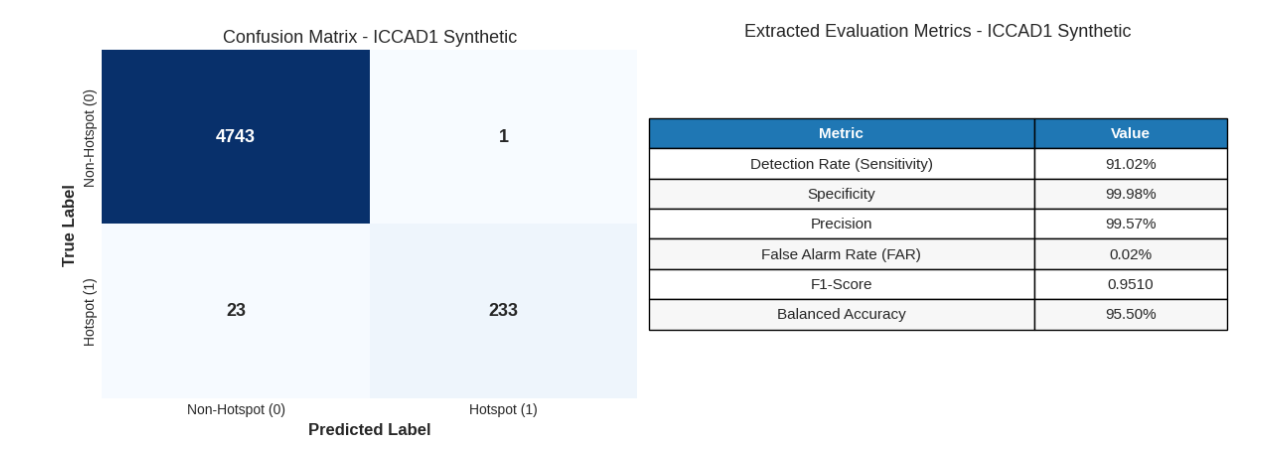
\includegraphics[width=\textwidth]{figures/image5.png}
\caption{Confusion matrix and extracted metrics on diagnostic fixture.}
\label{fig:val_cm}
\end{minipage}
\end{figure}

\begin{table}[htbp]
\caption{Evaluation Pipeline Diagnostic Metrics on \texttt{ICCAD1 Synthetic} Fixture}
\label{tab:pipeline_val}
\centering
\setlength{\tabcolsep}{2pt}
\begin{tabular}{p{0.43\columnwidth}cp{0.36\columnwidth}}
\toprule
\textbf{Metric} & \textbf{Value} & \textbf{Basis / Formulation} \\
\midrule
\textbf{Detection Rate (Sensitivity)} & 91.02\% & $\text{TP} = 233$ \\
\textbf{Specificity} & 99.98\% & $\text{TN} = 4,743$ \\
\textbf{Precision} & 99.57\% & $\text{FP} = 1$ \\
\textbf{False Alarm Rate} & 0.02\% & $\text{FN} = 23$ \\
\textbf{F1-Score} & 0.9510 & Harmonic mean \\
\textbf{Balanced Accuracy} & 95.50\% & $(\text{Sens} + \text{Spec})/2$ \\
\bottomrule
\end{tabular}
\end{table}

This diagnostic run proves that the evaluation calculations are mathematically self-consistent: with $\text{TP}=233$, $\text{FN}=23$, $\text{FP}=1$, and $\text{TN}=4,743$, Sensitivity is $233/256 = 91.02\%$, Precision is $233/234 = 99.57\%$, Specificity is $4,743/4,744 = 99.98\%$, Balanced Accuracy is $95.50\%$, and F1 is exactly:
\begin{equation}
\text{F1} = 2 \times \frac{0.995726 \times 0.910156}{0.995726 + 0.910156} = \frac{466}{490} \approx 0.9510
\end{equation}
This confirms arithmetic accuracy. We explicitly clarify that this diagnostic fixture was used solely for pipeline integration verification and must not be conflated with the real ICCAD-1 test partition (which contains 4,905 raw clips: 226 HS and 4,679 NHS).

\section{Ablation Studies}

\subsection{Test/Validation Leakage Discovery and Correction}
During initial development, the XAI training pipeline was found to map the validation directory directly to each benchmark's test folder, causing checkpoint selection to access the final evaluation split. This leakage was corrected by carving a stratified 15\% validation split from the training data with seed 42, holding out the test set for a single evaluation.

Table~\ref{tab:leakage} compares the XAI-ready CNN balanced accuracy before and after leakage correction. Clean splits caused balanced accuracy to decline on three benchmarks (ICCAD-1 by $-1.92$ pp, ICCAD-3 by $-1.32$ pp, and ICCAD-5 by $-5.32$ pp), while ICCAD-2 ($+5.27$ pp) and ICCAD-4 ($+1.04$ pp) improved, resulting in a net $-0.45$ pp shift across all benchmarks. ICCAD-5 exhibited the largest drop due to its minimal training population (26 HS clips). All primary XAI models in this paper utilize clean splits.

\subsection{Class-Imbalance Handling Ablation}
To investigate feature representations under extreme class imbalance, a controlled ablation was conducted on ICCAD-5 (train imbalance 104.5:1) comparing three conditions under identical architecture, optimizer, split, and seed: unweighted training, inverse-frequency class weighting ($w_{\text{HS}} = 52.73$), and balanced mini-batch sampling (16 HS / 16 NHS drawn with replacement).

\begin{table}[htbp]
\caption{ICCAD-5 Class-Imbalance Handling Ablation}
\label{tab:imbalance_ablation}
\centering
\setlength{\tabcolsep}{1.5pt}
\begin{tabular}{lcccc}
\toprule
\textbf{Condition} & \textbf{Bal.~Acc.} & \textbf{HS Recall} & \textbf{Zero-Vec} & \textbf{HS Units} \\
\midrule
\textbf{baseline\_noweight} & 0.9741 & 0.9512 & 0.0\% & 1 (AUC 0.982) \\
\textbf{class\_weighted} & 0.9649 & 0.9512 & 85.4\% & 0 \\
\textbf{balanced\_sampling} & 0.9501 & 0.9024 & 0.0\% & 4 (AUC 0.987) \\
\bottomrule
\end{tabular}
\end{table}

As reported in Table~\ref{tab:imbalance_ablation}, the loss-reweighted condition induced severe feature collapse: 85.4\% of penultimate-layer activations for hotspot test samples collapsed to all-zero vectors. In contrast, balanced mini-batch sampling completely eliminated feature collapse (0.0\% zero-vector rate) and produced four penultimate units with strong hotspot-elevated selectivity (AUC 0.97--0.99). A 3-seed replication (seeds 101, 202, 303) confirmed 0.0\% collapse for balanced sampling across all seeds, whereas the unweighted condition's non-collapse proved seed-dependent.

\section{Explainable AI: Multi-Method Analysis}

\subsection{Attribution Setup and Provenance Notice}
The explainability framework targets the \texttt{conv\_final\_2} feature map ($28\times28\times32$) of the XAI-ready CNN across four methods: Grad-CAM, closed-form Grad-CAM++, LayerCAM, and occlusion sensitivity. Grad-CAM++ uses the exact closed-form diagonal Hessian formulation of Chattopadhyay et al.~\cite{chattopadhyay2018} (Eqs. 19--21), resolving prior graph-recursion defects.

\textit{Provenance Notice:} The qualitative figures (Figs.~\ref{fig:case_hs123}--\ref{fig:case_nhs453}) and quantitative geometry metrics (Table~\ref{tab:geometry_xai}) were generated from the initial 57-sample evaluation cohort. To verify reproducibility on clean models, a suite of 20 clean TP/TN/FP/FN comparison figures and 60 raw float32 attribution arrays has been independently generated using the retrained clean checkpoints in \texttt{results/xai\_clean\_figures/}.

\subsection{Representative Case Studies}
The qualitative comparisons reveal pronounced method- and outcome-dependent behavior. For true-positive hotspots (Figs.~\ref{fig:case_hs123}--\ref{fig:case_hscad31012}), CAM attributions align closely with layout geometries and forward-pass occlusion sensitivity (e.g., LayerCAM reaches a Pearson correlation of 0.758 with occlusion on ICCAD-2). Conversely, on true-negative clips (Fig.~\ref{fig:case_nhs453}), Grad-CAM frequently concentrates on image boundaries or degenerates into uninformative maps.

\begin{figure*}[t]
\centering
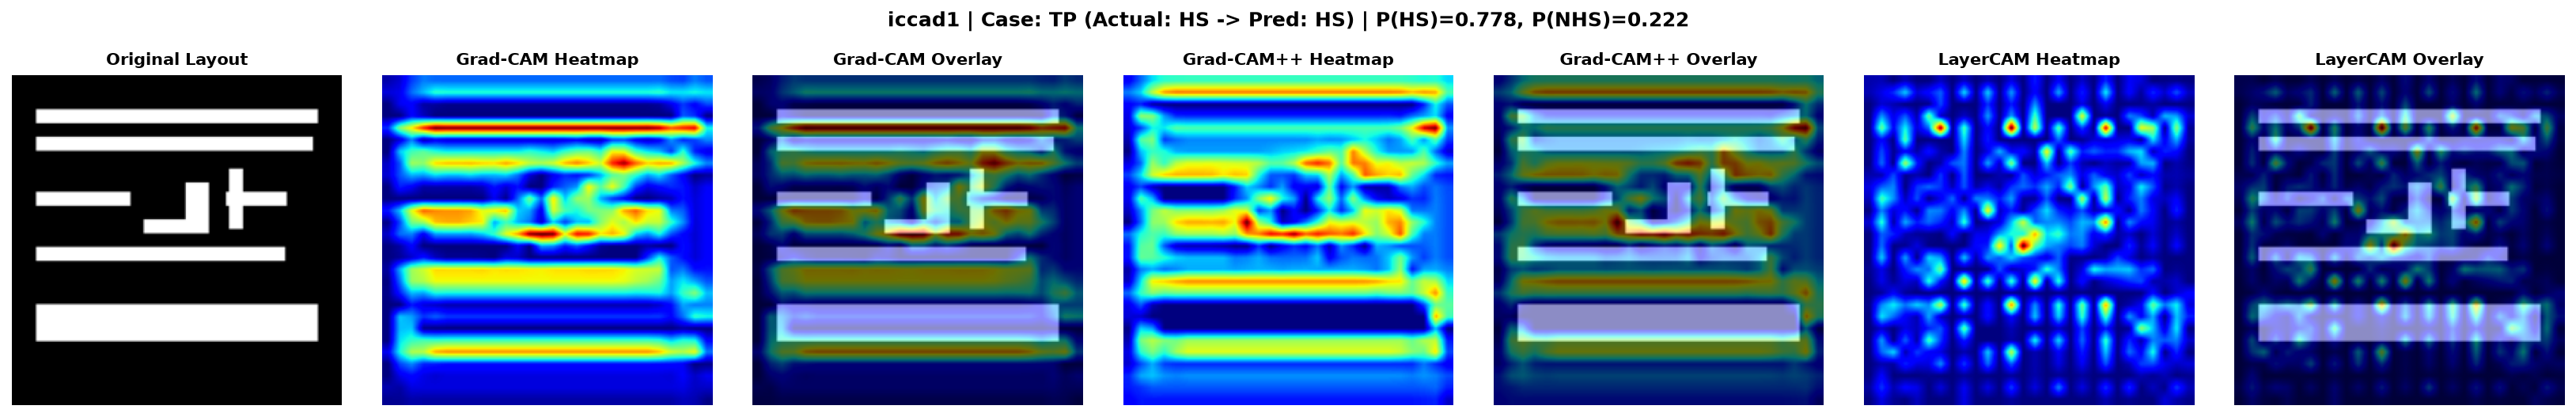
\includegraphics[width=0.96\textwidth]{figures/image7.png}
\vspace{-2mm}
\caption{ICCAD-1 HS123 (TP). Grad-CAM and Grad-CAM++ localize compactly, while LayerCAM highlights distributed features tracking layout structures.}
\label{fig:case_hs123}
\vspace{1.5mm}
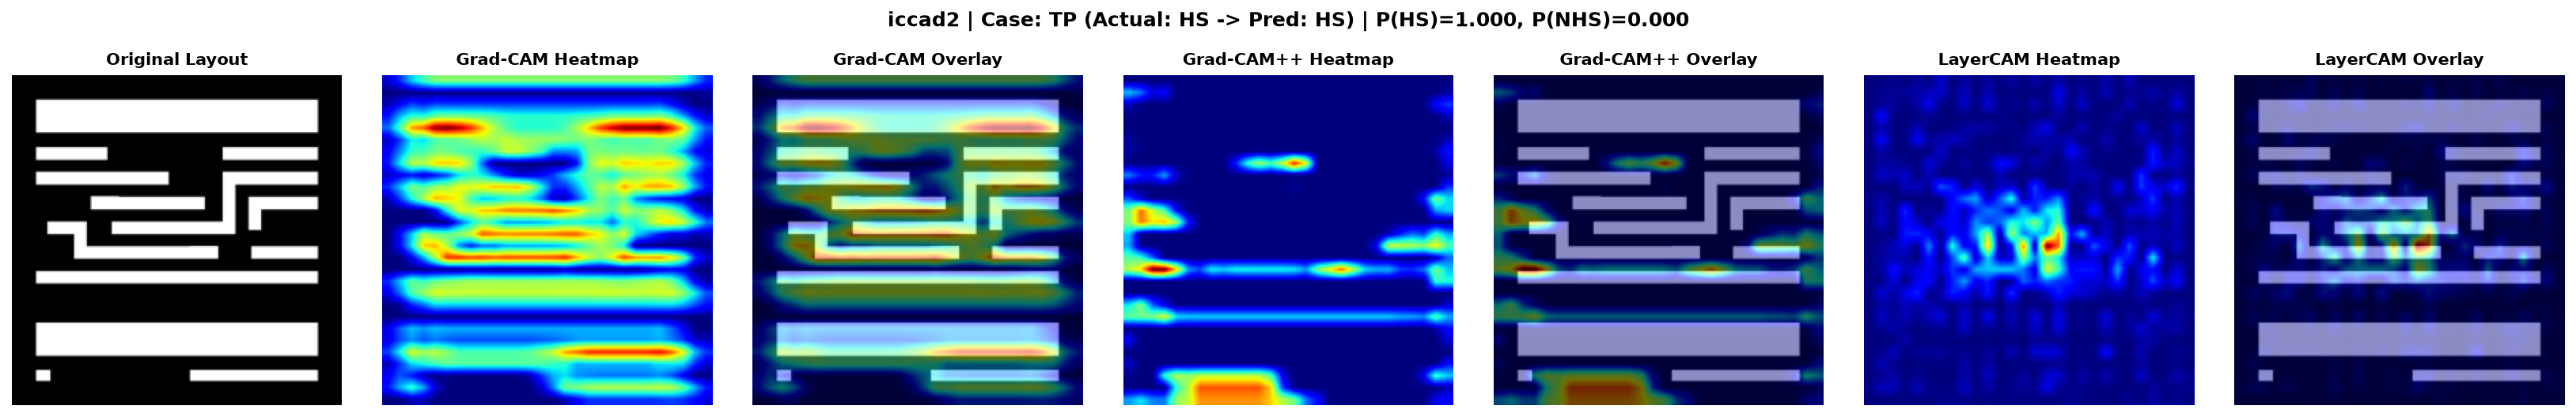
\includegraphics[width=0.96\textwidth]{figures/image8.png}
\vspace{-2mm}
\caption{ICCAD-2 HSCAD2146 (TP). Grad-CAM, Grad-CAM++, LayerCAM, and occlusion agree strongly; LayerCAM achieves $r = 0.758$ with occlusion.}
\label{fig:case_hscad2146}
\end{figure*}

\begin{figure*}[t]
\centering
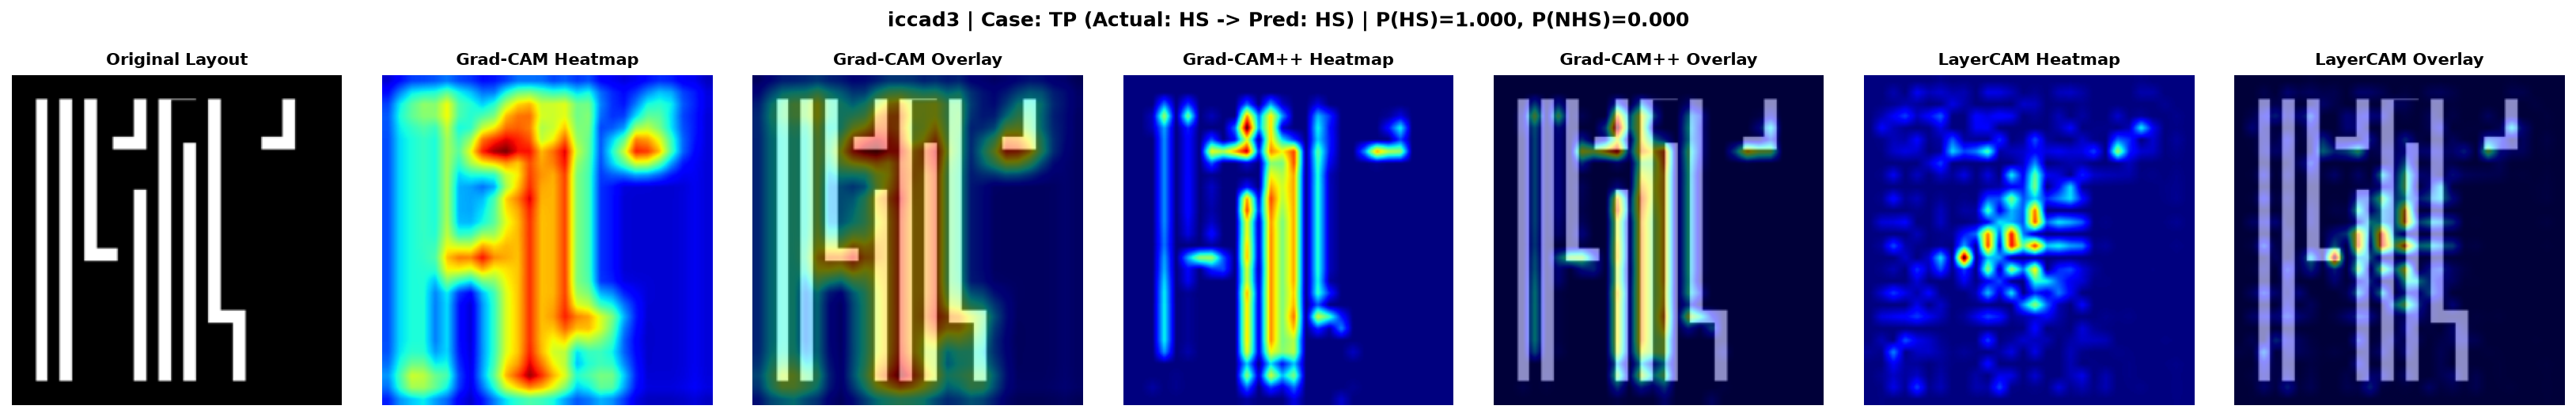
\includegraphics[width=0.96\textwidth]{figures/image9.png}
\vspace{-2mm}
\caption{ICCAD-3 HSCAD31012 (TP). All three CAM methods show strong positive correlation with the occlusion sensitivity reference ($r \approx 0.58$--$0.75$).}
\label{fig:case_hscad31012}
\vspace{1.5mm}
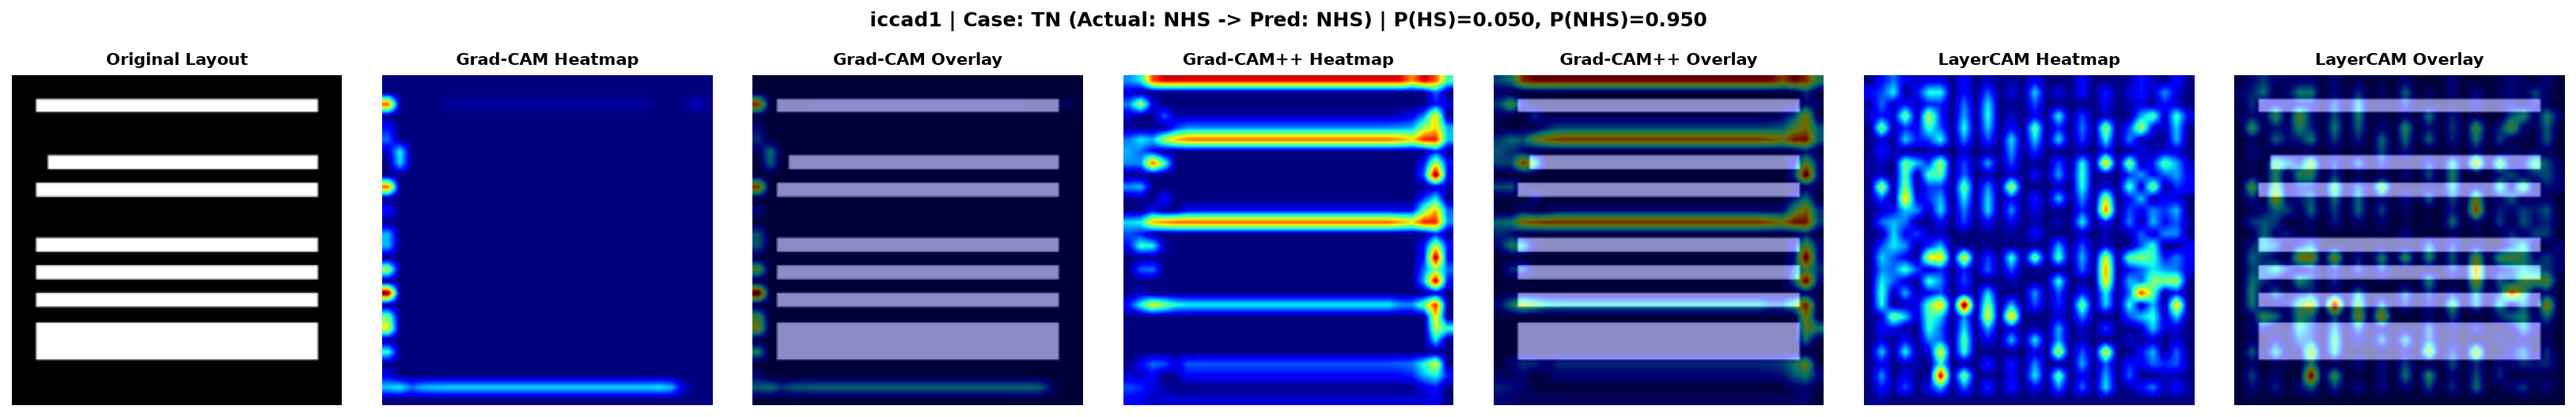
\includegraphics[width=0.96\textwidth]{figures/image10.png}
\vspace{-2mm}
\caption{ICCAD-1 NHS453 (TN). Grad-CAM shows edge-concentration artifact and lacks clear layout alignment despite correct NHS classification.}
\label{fig:case_nhs453}
\end{figure*}

\subsection{Quantitative 2D Raster-Morphology Validation}
Across the 57-sample cohort, the top-20\% attribution region of each method was compared against an area-matched random tile control using paired Wilcoxon signed-rank tests (30 random tile draws per sample; Table~\ref{tab:geometry_xai}).

\begin{table*}[t]
\caption{Geometry-Referenced Attribution Overlap vs. Area-Matched Control (57 Samples)}
\label{tab:geometry_xai}
\centering
\setlength{\tabcolsep}{3pt}
\begin{tabular}{p{0.13\textwidth}p{0.22\textwidth}p{0.24\textwidth}p{0.35\textwidth}}
\toprule
\textbf{Method} & \textbf{Median $\Delta$ Overlap vs. Control} & \textbf{Significance} & \textbf{Engineering Interpretation} \\
\midrule
\textbf{Grad-CAM} & $+0.033$ & $p=0.181$ (pooled); $p=0.022$ (TP) & Effective on TP hotspots; chance-level overall; below chance on TN \\
\textbf{Grad-CAM++} & $+0.047$ & $p=0.016$ (pooled) & Modest gain; TP-only effect not statistically significant \\
\textbf{LayerCAM} & $+0.108$ & $p<0.001$ (all groups) & Robust and consistent above-chance layout feature localization \\
\textbf{Occlusion} & $+0.164$ & $p<0.001$ (all groups) & Strongest layout sensitivity signal via direct forward masking \\
\bottomrule
\end{tabular}
\end{table*}

\textit{Qualification of Geometric Proxies:} Geometric layout features in Table~\ref{tab:geometry_xai} (corners, narrow gaps, thin lines) are extracted via 2D binary raster morphology (Sobel filters, Harris corner detection, morphological thinning). They represent structural layout pattern complexity rather than physical optical lithography aerial image simulations or foundry Design Rule Check (DRC) ground truth.

\subsection{Grad-CAM Degeneracy and Failure Modes}
Two distinct failure mechanisms were identified:
\begin{enumerate}
    \item \textbf{Feature Collapse:} Under severe class weighting on ICCAD-5, penultimate feature representations collapse to all-zero vectors, producing vanishing gradients and flat heatmaps across all gradient methods.
    \item \textbf{Gradient Cancellation:} On saturated logit predictions (e.g., ICCAD-3 sample NHSCAD31\_7 with logit $\approx 21.1$), gradient elements cancel during Grad-CAM's global average pooling, yielding zero post-ReLU activation. LayerCAM overcomes this by retaining pixel-level gradient weights.
\end{enumerate}
Across all 57 samples, exact flat-map rates reached 31.6\% for Grad-CAM, 42.1\% for Grad-CAM++, and only 8.8\% for LayerCAM.

\begin{figure*}[t]
\centering
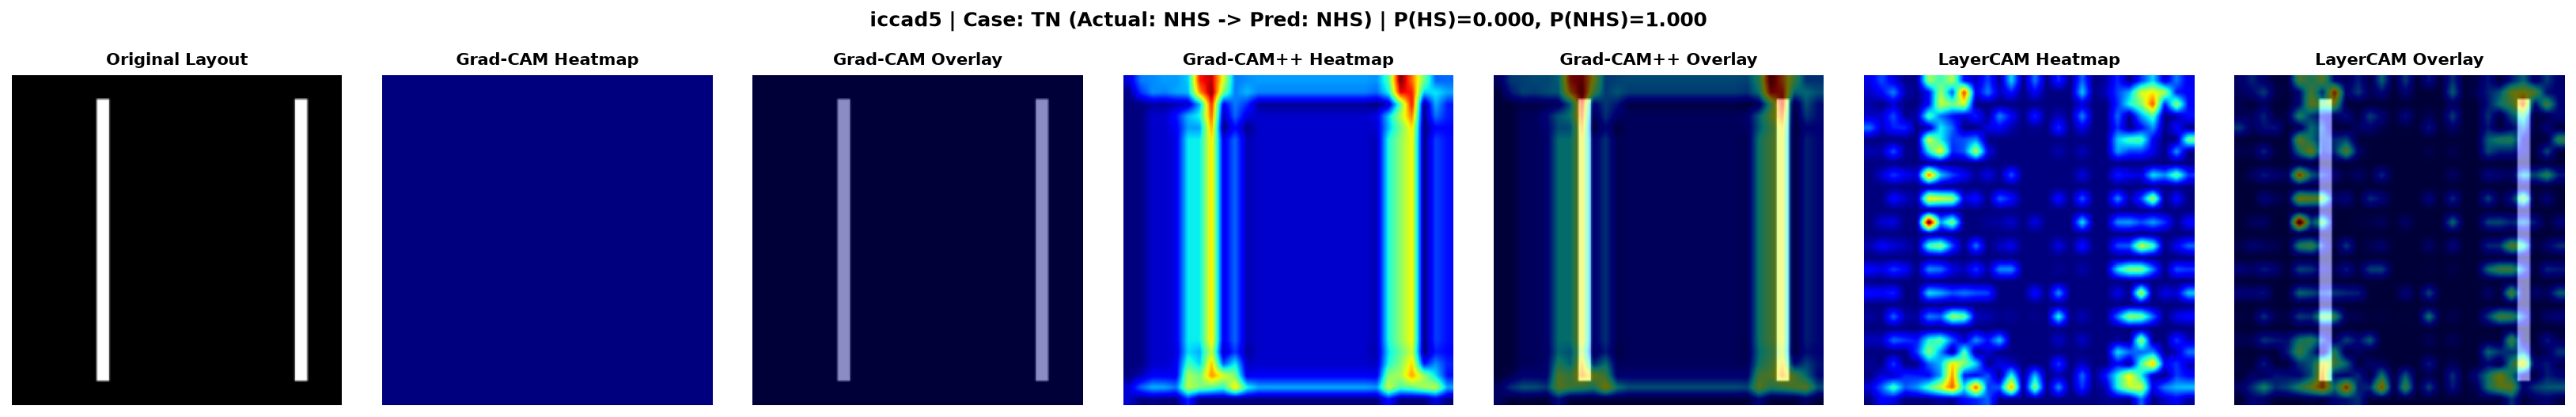
\includegraphics[width=0.96\textwidth]{figures/image11.png}
\vspace{-2mm}
\caption{ICCAD-5 NNHSCAD5999\_6 (TN): Grad-CAM and Grad-CAM++ degenerate to flat maps under penultimate feature collapse.}
\label{fig:case_iccad5_collapse}
\vspace{1.5mm}
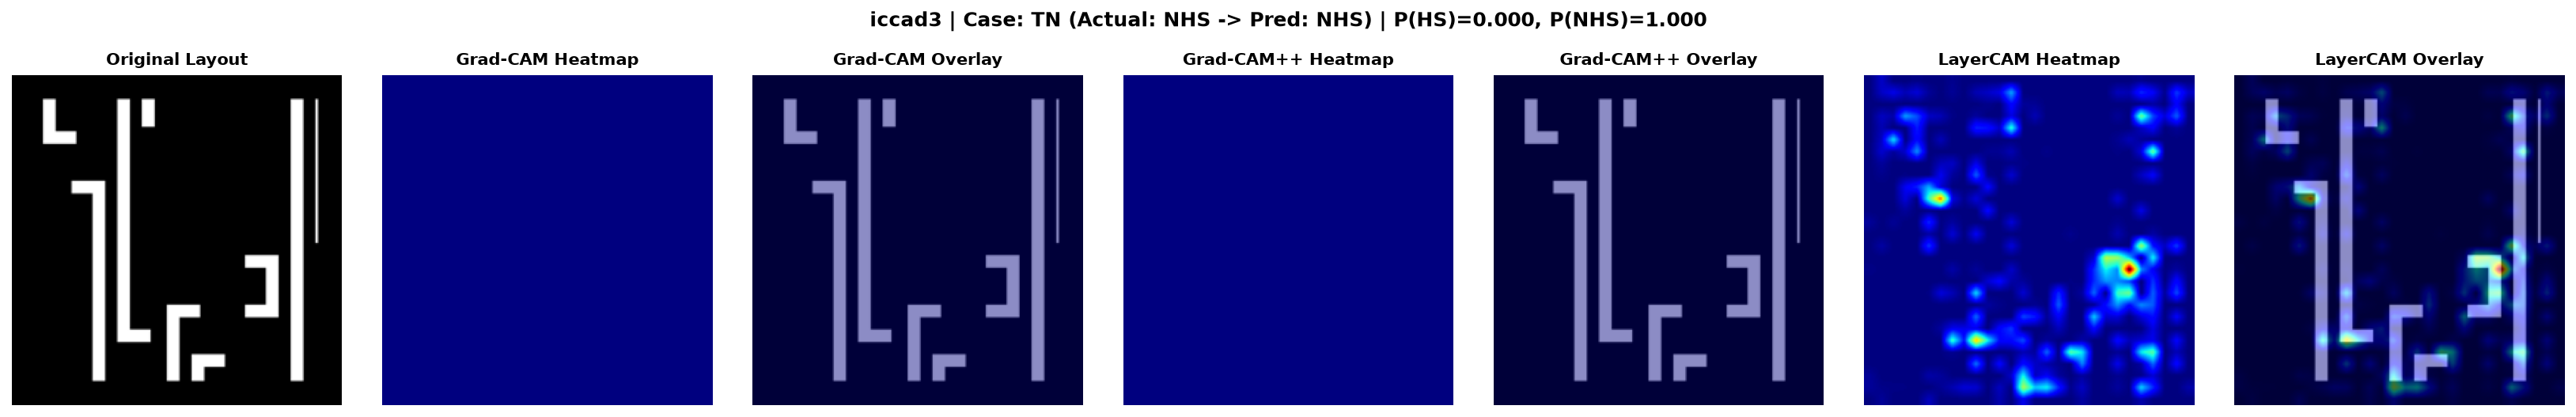
\includegraphics[width=0.96\textwidth]{figures/image12.png}
\vspace{-2mm}
\caption{ICCAD-3 NHSCAD31\_7 (TN): Grad-CAM flattens due to gradient cancellation under saturated logits, whereas LayerCAM preserves spatial structure.}
\label{fig:case_iccad3_saturation}
\end{figure*}

\subsection{Occlusion Cross-Check}
Occlusion sensitivity serves as a model-agnostic forward-pass reference. Across all 57 samples, median Pearson correlations with occlusion were 0.000 for Grad-CAM, 0.000 for Grad-CAM++, and 0.305 for LayerCAM (mean correlations: 0.080, 0.101, and 0.336). LayerCAM is the only CAM method exhibiting consistent positive alignment with forward sensitivity.

\subsection{Faithfulness, Sanity Checks, and Cross-Seed Stability}
Deletion and insertion AUC metrics were computed across held-out test clips for all five benchmarks (Table~\ref{tab:faithfulness}). LayerCAM achieves the lowest deletion AUC on four of five benchmarks and the highest insertion AUC on all five benchmarks (reaching 0.949 on ICCAD-3 and 0.946 on ICCAD-4).

\begin{table}[htbp]
\caption{XAI Faithfulness: Deletion / Insertion AUC on Held-Out Test Clips}
\label{tab:faithfulness}
\centering
\setlength{\tabcolsep}{3pt}
\begin{tabular}{lcccccc}
\toprule
 & \multicolumn{2}{c}{\textbf{Grad-CAM}} & \multicolumn{2}{c}{\textbf{Grad-CAM++}} & \multicolumn{2}{c}{\textbf{LayerCAM}} \\
\cmidrule(lr){2-3} \cmidrule(lr){4-5} \cmidrule(lr){6-7}
\textbf{Bench.} & Del $\downarrow$ & Ins $\uparrow$ & Del $\downarrow$ & Ins $\uparrow$ & Del $\downarrow$ & Ins $\uparrow$ \\
\midrule
\textbf{ICCAD-1} & 0.536 & 0.562 & 0.541 & 0.528 & \textbf{0.521} & \textbf{0.580} \\
\textbf{ICCAD-2} & 0.117 & 0.536 & 0.214 & 0.136 & \textbf{0.065} & \textbf{0.606} \\
\textbf{ICCAD-3} & 0.349 & 0.826 & 0.482 & 0.842 & \textbf{0.197} & \textbf{0.949} \\
\textbf{ICCAD-4} & 0.342 & 0.688 & 0.421 & 0.658 & \textbf{0.317} & \textbf{0.946} \\
\textbf{ICCAD-5} & \textbf{0.195} & 0.271 & 0.209 & 0.264 & 0.228 & \textbf{0.284} \\
\bottomrule
\end{tabular}
\end{table}

Adebayo parameter randomization tests confirm that attributions depend genuinely on learned network weights rather than acting as edge detectors (on ICCAD-5, Grad-CAM rank correlation with randomized weights drops to $r = -0.259$). Furthermore, cross-seed stability audits (seeds 101, 202, 303) show that LayerCAM maintains tight stability ($\text{SD} \le 0.084$), whereas Grad-CAM suffers high variance across seeds ($0.416 \pm 0.308$ on ICCAD-1).

\subsection{Direct Answer to the Research Question}
The findings yield a scientifically defensible, qualified yes: XAI techniques can localize layout regions contributing to hotspot classification, but attribution reliability depends critically on the method chosen and the classification outcome. LayerCAM and occlusion provide robust, statistically significant overlap with layout geometry across TP, TN, and FN outcomes. Conversely, Grad-CAM is reliable primarily for true-positive hotspot detections and degrades substantially on non-hotspots and collapsed checkpoints.

\section{Discussion and Limitations}
The central methodological conclusion is that explainability cannot be treated as a monolithic property. Relying solely on Grad-CAM risks false confidence due to unflagged flat maps and gradient cancellation.

A primary limitation is that geometric overlap is evaluated against 2D raster morphological proxies (corners, edges, line ends) rather than calibrated optical lithography aerial images (Abbe/Hopkins formulations) or foundry DRC rule violation coordinate logs.

Additionally, the class-weighted XAI model trades precision for recall in severely imbalanced benchmarks. Decision-threshold calibration on validation splits will be vital for operational deployment.

\section{Current Project Status and Future Work}
The project has successfully resolved core methodological deliverables:
\begin{enumerate}
    \item Strict 3-way train/validation/test split isolation verified by AST static analysis and test assertions;
    \item Clean-split retrained models and verified lossless float32 attribution arrays saved across all five benchmarks;
    \item Quantitative faithfulness verification via progressive deletion/insertion AUC, Adebayo weight randomization tests, and cross-seed stability audits;
    \item Exact closed-form Grad-CAM++ formulation; and
    \item 2D raster morphology statistical evaluations with 30 paired random tile controls.
\end{enumerate}

Future research priorities include validating geometric attributions against commercial DRC rule decks and physics-based optical lithography simulators, and extending multi-seed stability evaluations across ICCAD-3 and ICCAD-4.

\section{Conclusion}
This work evaluated CNN-based lithography hotspot detection and multi-method explainability across the five real ICCAD-12 benchmarks. By enforcing clean data isolation, correcting validation leakage, and systematically evaluating four XAI methods across 57 predictions and clean cohorts, we showed that LayerCAM and occlusion provide the most faithful and physically plausible layout attributions, whereas Grad-CAM requires careful monitoring for cancellation and collapse failure modes.

\section*{Project Repository and Artifacts}
Code, models, logs, and artifacts associated with this investigation are maintained in the project drive repository:
\url{https://drive.google.com/drive/folders/1_GFzS6NavQvI7Xn_FicbADCP6KV4_XBa?usp=sharing}

\balance

\begin{thebibliography}{00}

\bibitem{verma2026}
A.~Verma, K.~A.~Rao, and D.~S.~Hegde, ``Lithography Hotspot Detection using Deep Learning,'' Dept. of Electrical Engineering, IIT Bombay, India, reference paper provided for this assignment, 2026.

\bibitem{borisov2018}
V.~Borisov and J.~Scheible, ``Lithography Hotspots Detection Using Deep Learning,'' in \emph{Proc. 15th Int. Conf. on Synthesis, Modeling, Analysis and Simulation Methods and Applications to Circuit Design (SMACD)}, Prague, Czech Republic, 2018, pp.~145--148.

\bibitem{liao2022}
L.~Liao, S.~Li, Y.~Che, W.~Shi, and X.~Wang, ``Lithography Hotspot Detection Method Based on Transfer Learning Using Pre-Trained Deep Convolutional Neural Network,'' \emph{Appl. Sci.}, vol.~12, no.~4, p.~2192, 2022.

\bibitem{yang2017}
H.~Yang, Y.~Lin, B.~Yu, and E.~F.~Y.~Young, ``Lithography hotspot detection: From shallow to deep learning,'' in \emph{Proc. 30th IEEE Int. System-on-Chip Conf. (SOCC)}, Munich, Germany, 2017, pp.~233--238.

\bibitem{zhou2016}
B.~Zhou, A.~Khosla, A.~Lapedriza, A.~Oliva, and A.~Torralba, ``Learning Deep Features for Discriminative Localization,'' in \emph{Proc. IEEE Conf. on Computer Vision and Pattern Recognition (CVPR)}, 2016, pp.~2921--2929.

\bibitem{selvaraju2017}
R.~R.~Selvaraju, M.~Cogswell, A.~Das, A.~Vedantam, D.~Parikh, and D.~Batra, ``Grad-CAM: Visual Explanations from Deep Networks via Gradient-based Localization,'' in \emph{Proc. IEEE Int. Conf. on Computer Vision (ICCV)}, 2017, pp.~618--626.

\bibitem{jiang2025lithoexp}
C.~Jiang, H.~Sun, D.~Feng, Z.~Xie, B.~Tan, and K.~Liu, ``LithoExp: Explainable Two-stage CNN-based Lithographic Hotspot Detection with Layout Defect Localization,'' \emph{ACM Trans. on Design Automation of Electronic Systems}, vol.~30, no.~3, pp.~1--25, 2025.

\bibitem{chattopadhyay2018}
A.~Chattopadhyay, A.~Sarkar, P.~Howlader, and V.~N.~Balasubramanian, ``Grad-CAM++: Generalized Gradient-based Visual Explanations for Deep Convolutional Networks,'' in \emph{Proc. IEEE Winter Conf. on Applications of Computer Vision (WACV)}, 2018, pp.~839--847.

\bibitem{jiang2021layercam}
P.-T.~Jiang, C.-B.~Zhang, Q.~Hou, M.-M.~Cheng, and Y.~Wei, ``LayerCAM: Exploring Hierarchical Class Activation Maps for Localization,'' \emph{IEEE Trans. Image Processing}, vol.~30, pp.~5875--5888, 2021.

\end{thebibliography}

\end{document}
